\documentclass[12pt]{article}

\usepackage{amsmath,amsfonts,amssymb,mathtools}
\usepackage{physics,siunitx}
\usepackage{graphicx,subcaption,caption}
\usepackage[hidelinks]{hyperref}


\usepackage{color}


\usepackage[maxnames=2, style=phys,articletitle=true,biblabel=brackets,chaptertitle=false,pageranges=false,]{biblatex}

\addbibresource{references.bib}

\usepackage{abstract}
\usepackage[titletoc,page]{appendix}

\oddsidemargin=0in
\evensidemargin=0in
\textwidth=6.25in
\headsep=0pt
\headheight=0pt
\topmargin=0in
\textheight=9in

\usepackage[T1]{fontenc}
\usepackage[utf8]{inputenc}
\usepackage[swedish,english]{babel}


\setlength{\parindent}{0em}
\setlength{\parskip}{1em}


\begin{document}

\title{ALS}

\author{
    \begin{tabular}{c@{\hskip 1cm}c}
        Yue Jiao         & Mattias Jönsson \\
        \texttt{911024-7799} & \texttt{940425-0673} \\
        \texttt{yj@kth.se} & \texttt{matjon4@kth.se}
    \end{tabular}
    \vspace{0.5cm}\\
            SH1012 Modern Physics
}

\date{
    May 2, 2016
}

\maketitle

\section{Introduction}
Morse potential is a model used to describe intermolecular vibrations in diatomic molecules. The goal of this experiment is to measure the parameters in Morse potential for a $I_2$ gas. This will be done by excitation of $I_2$ molecules with a HeNe-laser and then measuring the florescent response from the $I_2$ gas.

\section{Theoretical background}
\subsection{Morse potential}
Morse potential is a model used to describe intermolecular vibrations. Unlike the harmonic oscillator, Morse potential has a reasonable physical behaviour far from equilibrium, which therefore makes it valid in a larger region. The potential is described by Morse function:
\begin{equation}
    V(r) = D_e \left(1-e^{\alpha(r_e-r)}\right)^2,
\end{equation}
where $D_e$ is the depth of the potential, $\alpha$ is a molecule specific constant, $r$ is the distance between the atoms and $r_e$ is the equilibrium distance.

\subsection{Vibrational energies}
From the Schrödinger equation with Morse potential we have that the eigenenergies are
\begin{equation}
    G(\nu) = \sum_{n=1}^\infty \omega_e k_n \left(\nu + \frac{1}{2} \right)^n,
    \label{G}
\end{equation}
where $\nu \in \mathbb{N}$ is the quantum number and $k_n$ is a constant with $k_1 = 1, k_2 = -x_e$. The total internal energy may then be expressed as
\begin{equation}
    T_{int} = T_{el} + G(\nu) + F(\nu),
    \label{T}
\end{equation}
where $T_{el}$ is the electronic energy and $F$ is the rotational energy. Equation \ref{G} and \ref{T} also applies for the excited state, however, we will denote it $\tilde{G}(\tilde{\nu})$ and $\tilde{T}_{int}$.

Let us introduce a new quantity the wavenumber $\sigma$, where $\sigma = 1/\lambda$. The laser excites the molecules to $\tilde{\nu} = 26$ so therefore
\begin{equation}
    \sigma(\nu) = \tilde{T}_{int}(\tilde{v} = 26) - T_{int}(\nu).
    \label{s}
\end{equation}
The difference between two wavenumbers can approximately be expressed as
\begin{equation}
    \sigma(\nu) - \sigma(\nu + 1) \approx G(\nu + 1) - G(\nu) \approx \omega_e - 2 \omega_e x_e (\nu + 1).
    \label{sigma}
\end{equation}

\subsection{Distance between wavelengths}
It is possible to show that the emitted wavelengths are equidistant by using equation \ref{sigma}:
\begin{equation}
    \frac{1}{\lambda(\nu)} - \frac{1}{\lambda(\nu + 1)} \approx \omega_e - 2 \omega_e x_e (\nu + 1) \implies \frac{1}{\lambda(\nu - 1)} + \frac{1}{\lambda(\nu + 1)} - \frac{2}{\lambda(\nu)} \approx 2 \omega_e x_e.
    \label{a}
\end{equation}
If we assume that $\omega_e x_e \approx 0$ equation \ref{a} gives:
\begin{equation}
        \frac{1}{\lambda(\nu - 1)} -  \frac{1}{\lambda(\nu)} \approx \frac{1}{\lambda(\nu + 1)} + \frac{1}{\lambda(\nu)} \iff
        \frac{\lambda(\nu) - \lambda(\nu - 1)}{\lambda(\nu - 1)\lambda(\nu)} \approx \frac{\lambda(\nu + 1) - \lambda(\nu)}{\lambda(\nu + 1)\lambda(\nu)}
\end{equation}
Let us further assume that $\frac{\lambda(\nu - 1)}{\lambda(\nu + 1)} \approx 1$ which implies
\begin{equation}
    \lambda(\nu) - \lambda(\nu - 1) \approx \lambda(\nu + 1) - \lambda(\nu)
\end{equation}

\subsection{Parameters in Morse potential}
The parameters in Morse potential may be calculated given that $\omega_e$, $x_e$, $\mu$ and $B_e$ is known. The parameters are calculated using the following equations.
\begin{equation}
    D_e \approx \frac{\omega_e^2}{4x_e\omega_e}
\end{equation}
\begin{equation}
    \alpha = 2\pi \sqrt{\frac{2x_e\omega_ec\mu}{h}}
\end{equation}
\begin{equation}
    r_e = \frac{1}{2\pi} \sqrt{\frac{h}{cmB_e}}
\end{equation}

\subsection{Single wavelength in spectrograph}
\label{secondpeak}
When measuring a single wavelength it is expected that the measured spectrum should have only one peak, however, this is not true for all wavelengths. The reason is that the spectrograph uses diffraction to split the incoming light into its corresponding wavelengths. By letting the incoming light beam bounces of a grating, the light beam will be phase-shifted differently dependent on where it bounced. This will create a phase difference in the light beam causing it to cancel out if the phase difference is equal to $(k+1/2)\lambda$, where $k \in \mathbb{N}$. If the phase difference is $k\lambda$ it will interfere constructively. So dependent on wavelength the light will interfere constructively at different reflection angles. The location of the maxima is described by Bragg's law:
\begin{equation}
    n\lambda = 2d\sin{\theta},
\end{equation}
where $n \in \mathbb{N}\backslash \{0\}$ corresponds to the order of the maximum, $\lambda$ is the wavelength, $d$ is the distance between the two planes in the grating and $\theta$ is the angle to the maximum. It is possible to find more than one angle where constructive interference occurs, which explains why there might be more than one peak in the spectrum. Since the spectrograph only measures the angle we therefore know that all peaks must correspond to $n\lambda$ and therefore will the second peak correspond to the double wavelength.

\section{Experimental setup}
\subsection{Material}
The equipment used in this experiment was a spectrograph, a HeNe-laser, a lens and a glass tube with $I_2$ gas. To calibrate the spectrograph a mirror and Hg-filters were used. The Hg-filters were each transparent to the wavelengths $4047$, $4358$, $5461$ and $5782$ respectively.

\subsection{Calibration}
The calibration of the spectrograph was conducted using light of known wavelengths. This was done by using light from the ceiling lamp, bouncing the light of a mirror to make it travel in the horizontal direction and making it pass through a lens and then a Hg filter. The filter only allows one wavelength to pass through it and the peak on the spectrograph was paired with the wavelength. For some Hg-filters a second peak was detected. The second peak was paired with the double wavelength as described in section \ref{secondpeak}. From a set of known wavelengths a polynomial was fit using the least-square method.


\subsection{Laser spectroscopy}
The spectrograph was set to average $50$ measurements with an exposure of $1.3 s$. With the laser turned off the background signal was measured. The background signal was set as the baseline for any further measurements. The laser was switched on and the florescent light was focused on the opening of the spectrograph. Each peak in the resulting spectrum was then recorded

The corresponding wavelengths for the peaks were calculated. Each consecutive wavelength $\sigma(\nu + 1) - \sigma(\nu)$ was calculated and plotted in a graph. Additional wavelengths were added where $\sigma(\nu + 1) - \sigma(\nu)$ approximately twice the visible line.

\pagebreak
\section{Results}
\subsection{Calibration}
\begin{figure}[ht]
    \centering
    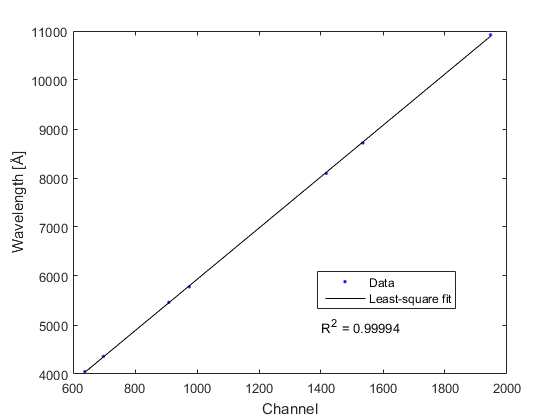
\includegraphics[width=0.7\textwidth]{calibration}
    
    \caption{The calibration of the spectrograph. Dots are data points and the line is the least-square fit.}
    \label{figure:calibration}
\end{figure}

Using the $7$ data points presented as dots in figure \ref{figure:calibration} to least-square fit a polynomial $P \in \mathbb{P}_1$ resulted in
\begin{equation}
  \lambda(c) = 689.9 + 5.241c,
\end{equation}
where $\lambda$ is the wavelength and $c$ is the channel number. The coefficient of determination for this fit is $R^2 = 0.99994$. The data points are presented in table \ref{table:calibration}.

\begin{table}
\centering
\begin{tabular}{| c | c | }
    \hline
    Channel & Wavelength [Å] \\ \hline
    638 & 4047 \\ \hline
    698 & 4358 \\ \hline
    909 & 5461 \\ \hline
    975 & 5780 \\ \hline
    1417 & 8094 \\ \hline
    1535 & 8716 \\ \hline
    1947 & 10922 \\ \hline
\end{tabular}
\caption{Data from the calibration.}
\label{table:calibration}
\end{table}

\subsection{Laser spectroscopy}
The measured wavelengths are presented in table \ref{table:data} and the corresponding $\Delta G = \sigma(\nu + 1) - \sigma(\nu)$ values are plotted in figure \ref{figure:curve}. The $\Delta G$ are fitted with a linear model with $R = 0.5496$. The experimental parameters in Morse potential is calculated using $\omega_e$ and $\omega_ex_e$ from this experiment and $B_e$ from NIST~\cite{NIST}. The reference parameters are calculated from values the NIST values of $\omega_e$ and $\omega_ex_e$. The values are presented in table \ref{table:data} and the parameters are presented in table \ref{table:values}

\begin{table}[ht]
\centering
\begin{tabular}{| c | c | c | }
    \hline
    $\nu$ & Wavelength [Å] & $\Delta G$ [cm^-1] \\ \hline
    0   &   5448    &   157.5 \\ \hline
    1   &   5496    &   239.7 \\ \hline
    2   &   5569    &	233.5 \\ \hline
    3   &   5642    &   211.4 \\ \hline
    {\color{red} 4}   &   {\color{red}5710}	&	{\color{red}206.5} \\ \hline
    5   &   5779    &   209.3 \\ \hline
    6   &   5849	&	204.3 \\ \hline
    7   &   5920    &   235.9 \\ \hline
    8   &   6004	&	186.9 \\ \hline
    {\color{red} 9}   &   {\color{red}6072}	&	{\color{red}182.7} \\ \hline
    10  &   6140	&	212.6 \\ \hline
    {\color{red} 11}   &   {\color{red}6221}	&	{\color{red}207.2} \\ \hline
    12  &   6303	&	189.0 \\ \hline
    13  &   6379	&	184.6 \\ \hline
    14  &   6455	&	223.2 \\ \hline
    15  &   6549	&	193.0 \\ \hline
    16  &   6633	&	176.6 \\ \hline
    17  &   6711	&	195.2 \\ \hline
    {\color{red} 18}   &   {\color{red}6800}	&	{\color{red}190.2} \\ \hline
    19  &   6890	&	179.9 \\ \hline
    {\color{red} 20}   &   {\color{red}6976}	&	{\color{red}175.5} \\ \hline
    21  &   7062	&	217.3 \\ \hline
    22  &   7173	&	161.1 \\ \hline
    23  &   7256	&	186.5 \\ \hline
    24  &   7356	&	181.6 \\ \hline
    {\color{red} 25}   &   {\color{red}7456}	&	{\color{red}176.8} \\ \hline
    26  &   7555	&	172.2 \\ \hline
    {\color{red} 27}   &   {\color{red}7655}	&	{\color{red}167.8} \\ \hline
    28  &   7754    &	172.0 \\ \hline
    29  &   7859    &   - \\ \hline
    
\end{tabular}
\caption{Data from the laser spectroscopy measurement. Red values are interpolated. $\Delta G = \sigma(\nu + 1) - \sigma(\nu)$}
\label{table:data}
\end{table}

\begin{table}[ht]
\centering
\begin{tabular}{| c | c | c | c | }
    \hline
    Parameter & Experimental value & Reference value & Relative error \\ \hline
    $\omega_e$ & $225.4 cm^-1$ & $214.5 cm^-1$ & $0.051$ \\ \hline
    $\omega_ex_e$ & $0.968$ & $0.614$ & $0.57$ \\ \hline
    $D_e$ & $1.31\cdot10^4 cm^-1$ &  $1.87 \cdot 10^4$ & $-0.29$ \\ \hline
    $\alpha$ & $1.91\cdot10^8 cm^-1$ & $1.52\cdot10^8 cm^-1$ & $0.25$ \\ \hline
    $r_e$ &  - & $2.666 Å$ & - \\ \hline
\end{tabular}
\caption{Morse potential parameters}
\label{table:values}
\end{table}

\begin{figure}[ht]
    \centering
    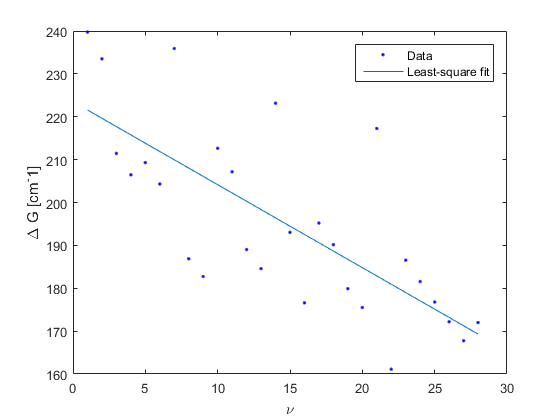
\includegraphics[width=0.7\textwidth]{curve}
    
    \caption{$\Delta G = \sigma(\nu + 1) - \sigma(\nu)$ plotted with a least-square fit. $R^2 = 0.5496$}
    \label{figure:curve}
\end{figure}

\pagebreak
\subsection{Morse potential}
In figure \ref{figure:morse} Morse potential is plotted using the experimental values and the reference values.
\begin{figure}[ht]
    \centering
    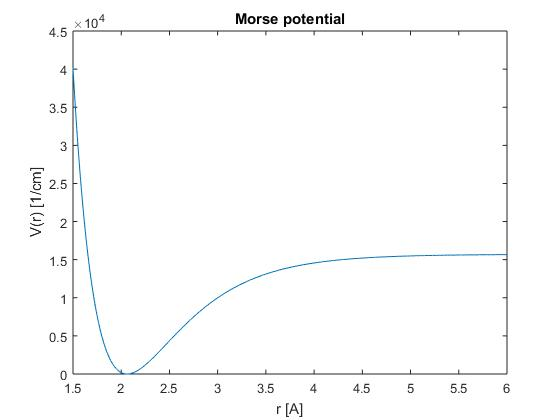
\includegraphics[width=0.6\textwidth]{morse}
    
    \caption{Experimental Morse potential in blue, reference potential in orange.}
    \label{figure:morse}
\end{figure}

\pagebreak
\section{Discussion}
The errors in $\omega_e$ and $\omega_ex_e$ are the most interesting since the other parameters are derived from those. From table \ref{table:values} we have that the relative error in $\omega_e$ is much smaller than the relative error in $\omega_ex_e$. Since $\omega_ex_e \ll \omega_e$ this means that the y-interception is well known compared to the slope of the curve. 

An error source is that we neglected the rotational energies in equation \ref{s}. We expect the error from this approximation to be rather small since the rotational energies are approximately two orders of magnitude smaller than the vibrational energies this error should be small. This, however, will increase the uncertainty in the measurement.

A second error source is the linearization of equation \ref{sigma}. Equation \ref{G} is a infinite sum, yet only the linear terms are used in the calculation. This will contribute to the error and increase the uncertainty given that not all higher order terms are zero.

A third error source is the resolution of the spectrograph. The spectrograph has limited resolution since it has 2048 discrete channels in which the incoming light is measured. Another factor that will affect the resolution negatively is that the light is not perfectly colimated and that the light does not necessarily enter at a right angle. The lower resolution will increase the uncertainty.

A fourth error source is the existence of a background signal. The spectrograph was base-lined with the background signal from the ambient light, but there could still be other types of background signals. For example is it possible that random fluctuations in the electronics caused background noise.

\printbibliography

\end{document}
